\documentclass{article}\usepackage[]{graphicx}\usepackage[]{xcolor}
% maxwidth is the original width if it is less than linewidth
% otherwise use linewidth (to make sure the graphics do not exceed the margin)
\makeatletter
\def\maxwidth{ %
  \ifdim\Gin@nat@width>\linewidth
    \linewidth
  \else
    \Gin@nat@width
  \fi
}
\makeatother

\definecolor{fgcolor}{rgb}{0.345, 0.345, 0.345}
\newcommand{\hlnum}[1]{\textcolor[rgb]{0.686,0.059,0.569}{#1}}%
\newcommand{\hlsng}[1]{\textcolor[rgb]{0.192,0.494,0.8}{#1}}%
\newcommand{\hlcom}[1]{\textcolor[rgb]{0.678,0.584,0.686}{\textit{#1}}}%
\newcommand{\hlopt}[1]{\textcolor[rgb]{0,0,0}{#1}}%
\newcommand{\hldef}[1]{\textcolor[rgb]{0.345,0.345,0.345}{#1}}%
\newcommand{\hlkwa}[1]{\textcolor[rgb]{0.161,0.373,0.58}{\textbf{#1}}}%
\newcommand{\hlkwb}[1]{\textcolor[rgb]{0.69,0.353,0.396}{#1}}%
\newcommand{\hlkwc}[1]{\textcolor[rgb]{0.333,0.667,0.333}{#1}}%
\newcommand{\hlkwd}[1]{\textcolor[rgb]{0.737,0.353,0.396}{\textbf{#1}}}%
\let\hlipl\hlkwb

\usepackage{framed}
\makeatletter
\newenvironment{kframe}{%
 \def\at@end@of@kframe{}%
 \ifinner\ifhmode%
  \def\at@end@of@kframe{\end{minipage}}%
  \begin{minipage}{\columnwidth}%
 \fi\fi%
 \def\FrameCommand##1{\hskip\@totalleftmargin \hskip-\fboxsep
 \colorbox{shadecolor}{##1}\hskip-\fboxsep
     % There is no \\@totalrightmargin, so:
     \hskip-\linewidth \hskip-\@totalleftmargin \hskip\columnwidth}%
 \MakeFramed {\advance\hsize-\width
   \@totalleftmargin\z@ \linewidth\hsize
   \@setminipage}}%
 {\par\unskip\endMakeFramed%
 \at@end@of@kframe}
\makeatother

\definecolor{shadecolor}{rgb}{.97, .97, .97}
\definecolor{messagecolor}{rgb}{0, 0, 0}
\definecolor{warningcolor}{rgb}{1, 0, 1}
\definecolor{errorcolor}{rgb}{1, 0, 0}
\newenvironment{knitrout}{}{} % an empty environment to be redefined in TeX

\usepackage{alltt}
\usepackage{amsmath} %This allows me to use the align functionality.
                     %If you find yourself trying to replicate
                     %something you found online, ensure you're
                     %loading the necessary packages!
\usepackage{amsfonts}%Math font
\usepackage{graphicx}%For including graphics
\usepackage{hyperref}%For Hyperlinks
\usepackage[shortlabels]{enumitem}% For enumerated lists with labels specified
                                  % We had to run tlmgr_install("enumitem") in R
\hypersetup{colorlinks = true,citecolor=black} %set citations to have black (not green) color
\usepackage{natbib}        %For the bibliography
\setlength{\bibsep}{0pt plus 0.3ex}
\bibliographystyle{apalike}%For the bibliography
\usepackage[margin=0.50in]{geometry}
\usepackage{float}
\usepackage{multicol}

%fix for figures
\usepackage{caption}
\newenvironment{Figure}
  {\par\medskip\noindent\minipage{\linewidth}}
  {\endminipage\par\medskip}
\IfFileExists{upquote.sty}{\usepackage{upquote}}{}
\begin{document}

\vspace{-1in}
\title{Lab 10 -- MATH 240 -- Computational Statistics}

\author{
  Yuliia Heleveria \\
  MATH 240  \\
  Colgate University  \\
  {\tt yheleveria@colgate.edu}
}

\date{02/08/2025}

\maketitle

\begin{multicols}{2}
\raggedcolumns % If your spacing gets messed up try uncommenting 
                % this line
\begin{abstract}
This document provides a basic template for the 2-page labs we will complete each week. Here, briefly summarize what you did and why it might be helpful. Provide all the top-line conclusions, but avoid providing \emph{all} the details. Results should be limited to ``we show X, Y, and Z."
\end{abstract}

\noindent \textbf{Keywords:} Margin of Error; Sample Size; Simulation; Resampling.

\section{Introduction}

Gallup polls published a document called ``\textit{How Are Polls Conducted}'' that describes how Gallup selects people to include in its polls. In the article, Gallup polls claimed that with a sample size of 1,000 national adults (derived with random selection procedures), the results are likely to be accurate within a margin of error of  $\pm$4 \% percentage points. Gallup also concluded that if they increase a poll sample size to 2,000, the results then would be accurate within $\pm$2 \% of the underlying population value. 

In this lab, we aim to test if doubling the sample size, as Gallup claims, would actually decrease the margin of error in half. We performed basic simulation and resampling of a poll to test if modifying sample size would decrease the margin of error in half. Also, we experimented if varying other factors, such as the actual population proportion, would affect the margin of error.

Provide a roadmap of the structure of the paper. 



\section{Methods}
We take conclude that the margin of error provides 95\% confidence. As a example study, we chose to replicate poll results of February 3-16, 2025 poll of 1,004 adults aged 18+ living in all 50 U.S. states and the District of Columbia about their satisfaction with position of the United States in the world today. The results revealed that 39\% of respondents were satisfied, 59\% were dissatisfied, and 2\% had no opinion. Gallup reported margin of error of  $\pm$4 \% percentage points for this poll.

To begin, we conducted a basic simulation study with assumed population probability proportion $p=0.39$ for sample size $n=1004$ and then $n=2008$ to compare their estimated margin of error by halving the middle 95\%. We generated 10k polls for each sample size. 

\begin{Figure}
 \centering
 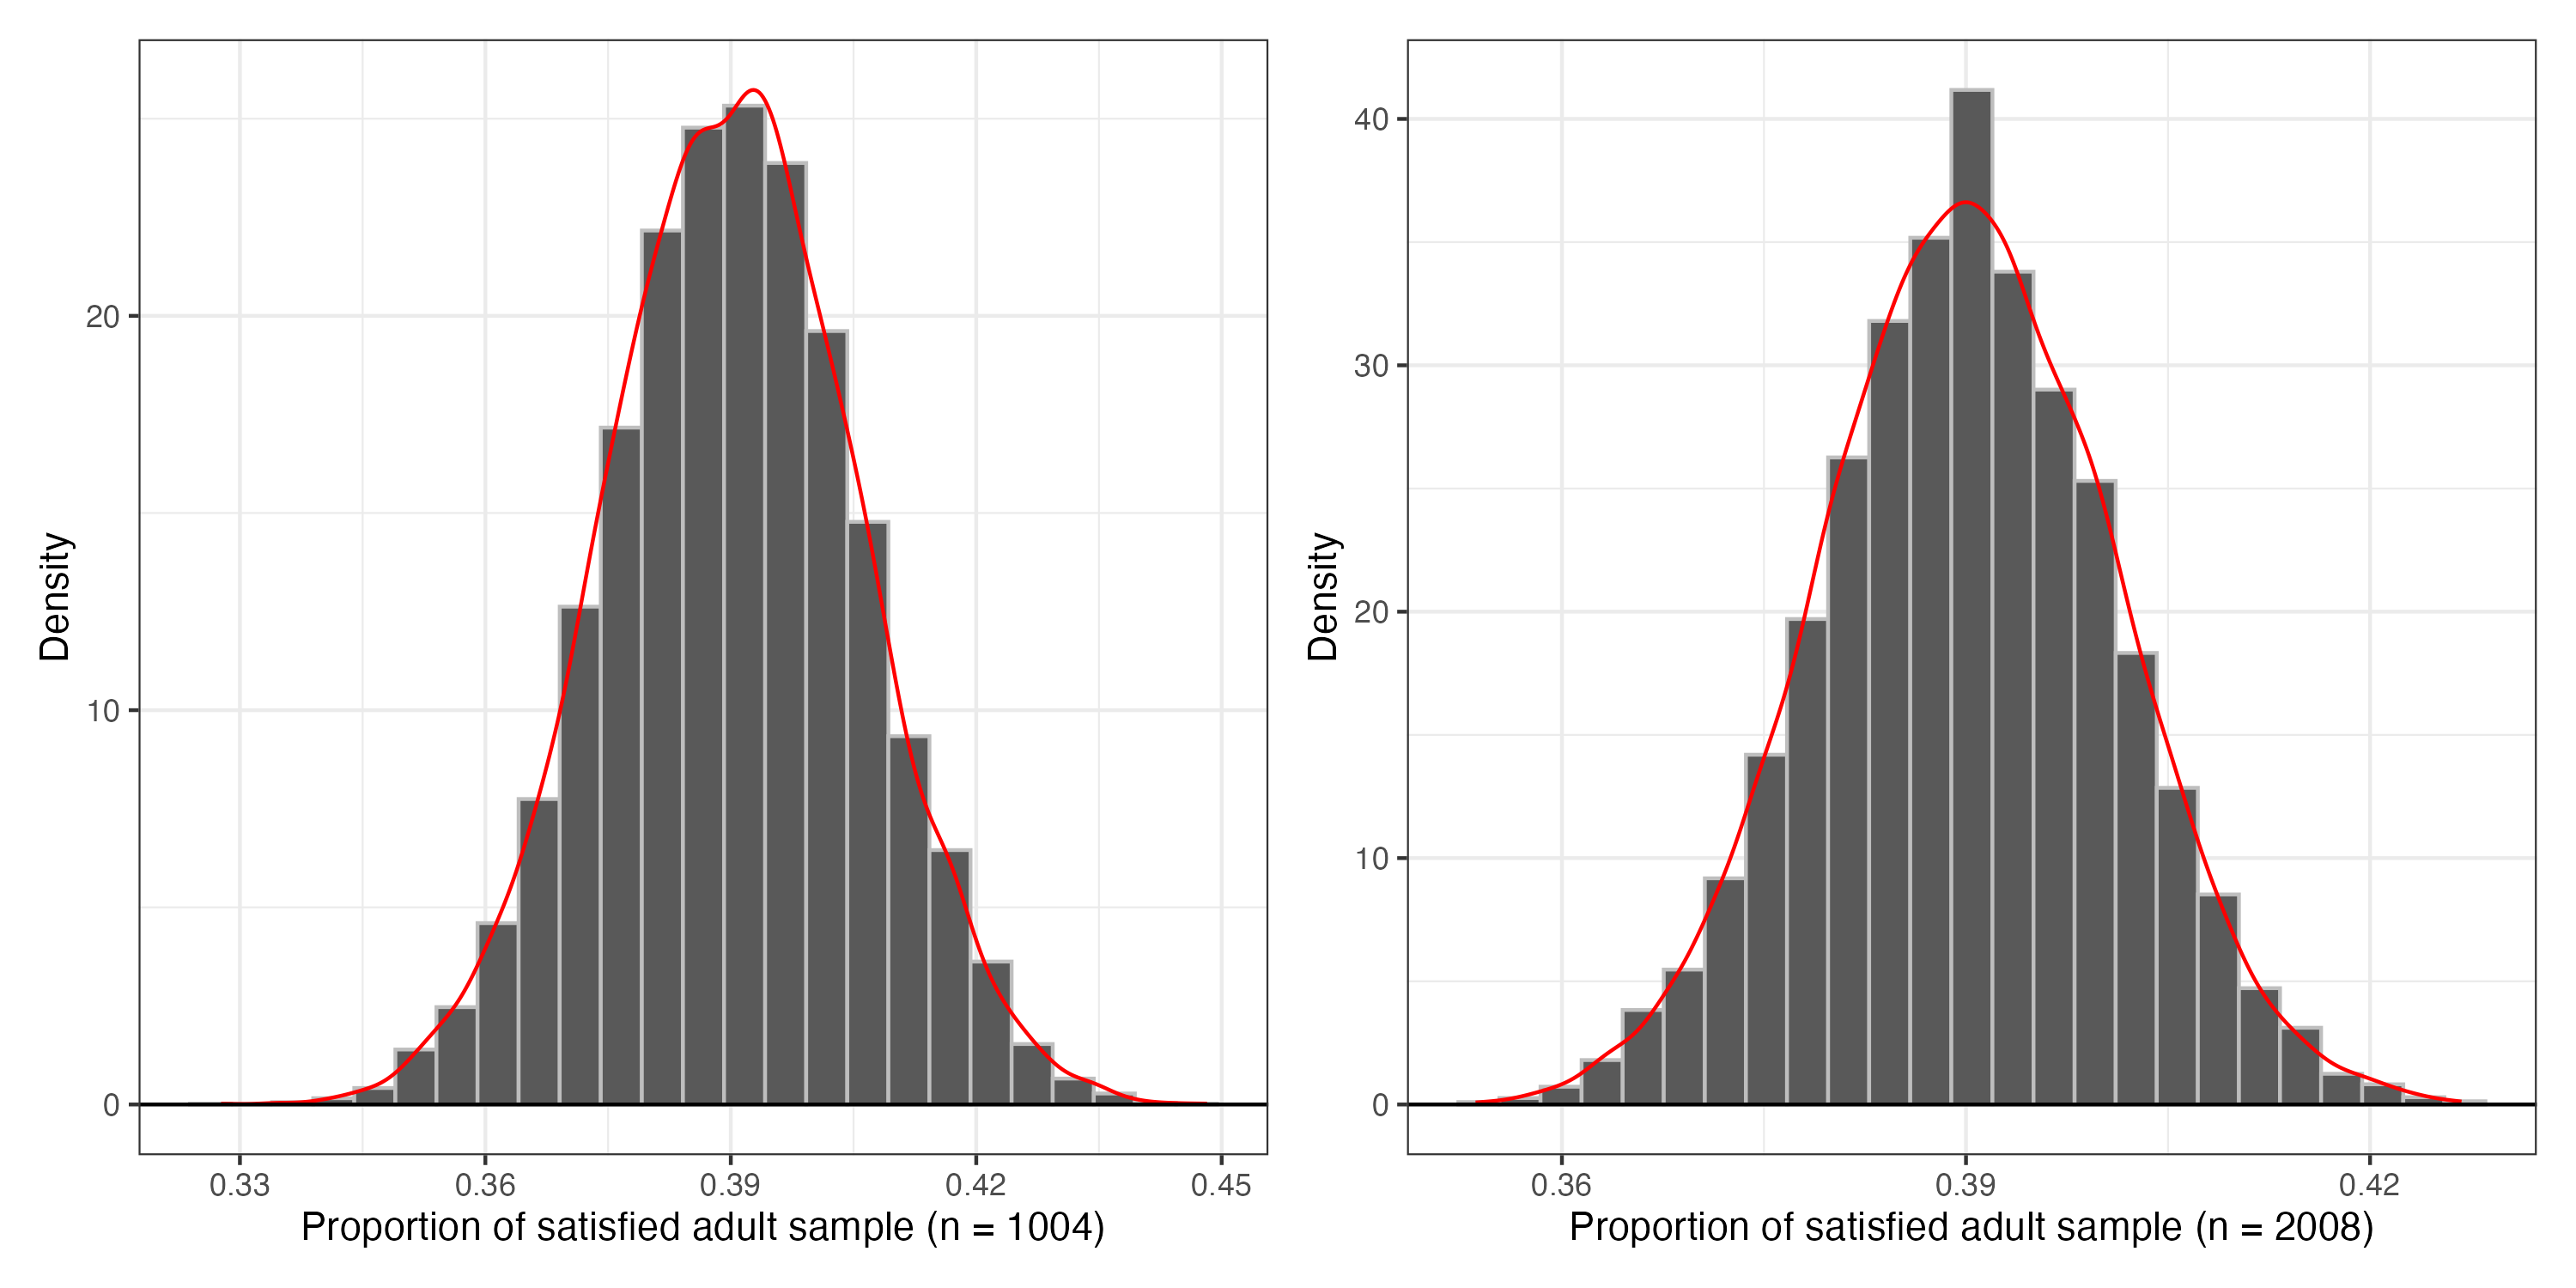
\includegraphics[width=\linewidth]{simulation.png}
 \captionof{figure}{Histogram of sample proportions with superimposed density}
 \label{fig:sim}
\end{Figure}

Another option for approximating the estimated error is resampling. We took random sample with replacement from the original sample 1000 times to reproduce the experiment on the population. For each random sample taken from the original, we calculated the mean. We then summarized the range of the middle 95\% of values, calculating the margin of error by halving the interval.

\begin{Figure}
 \centering
 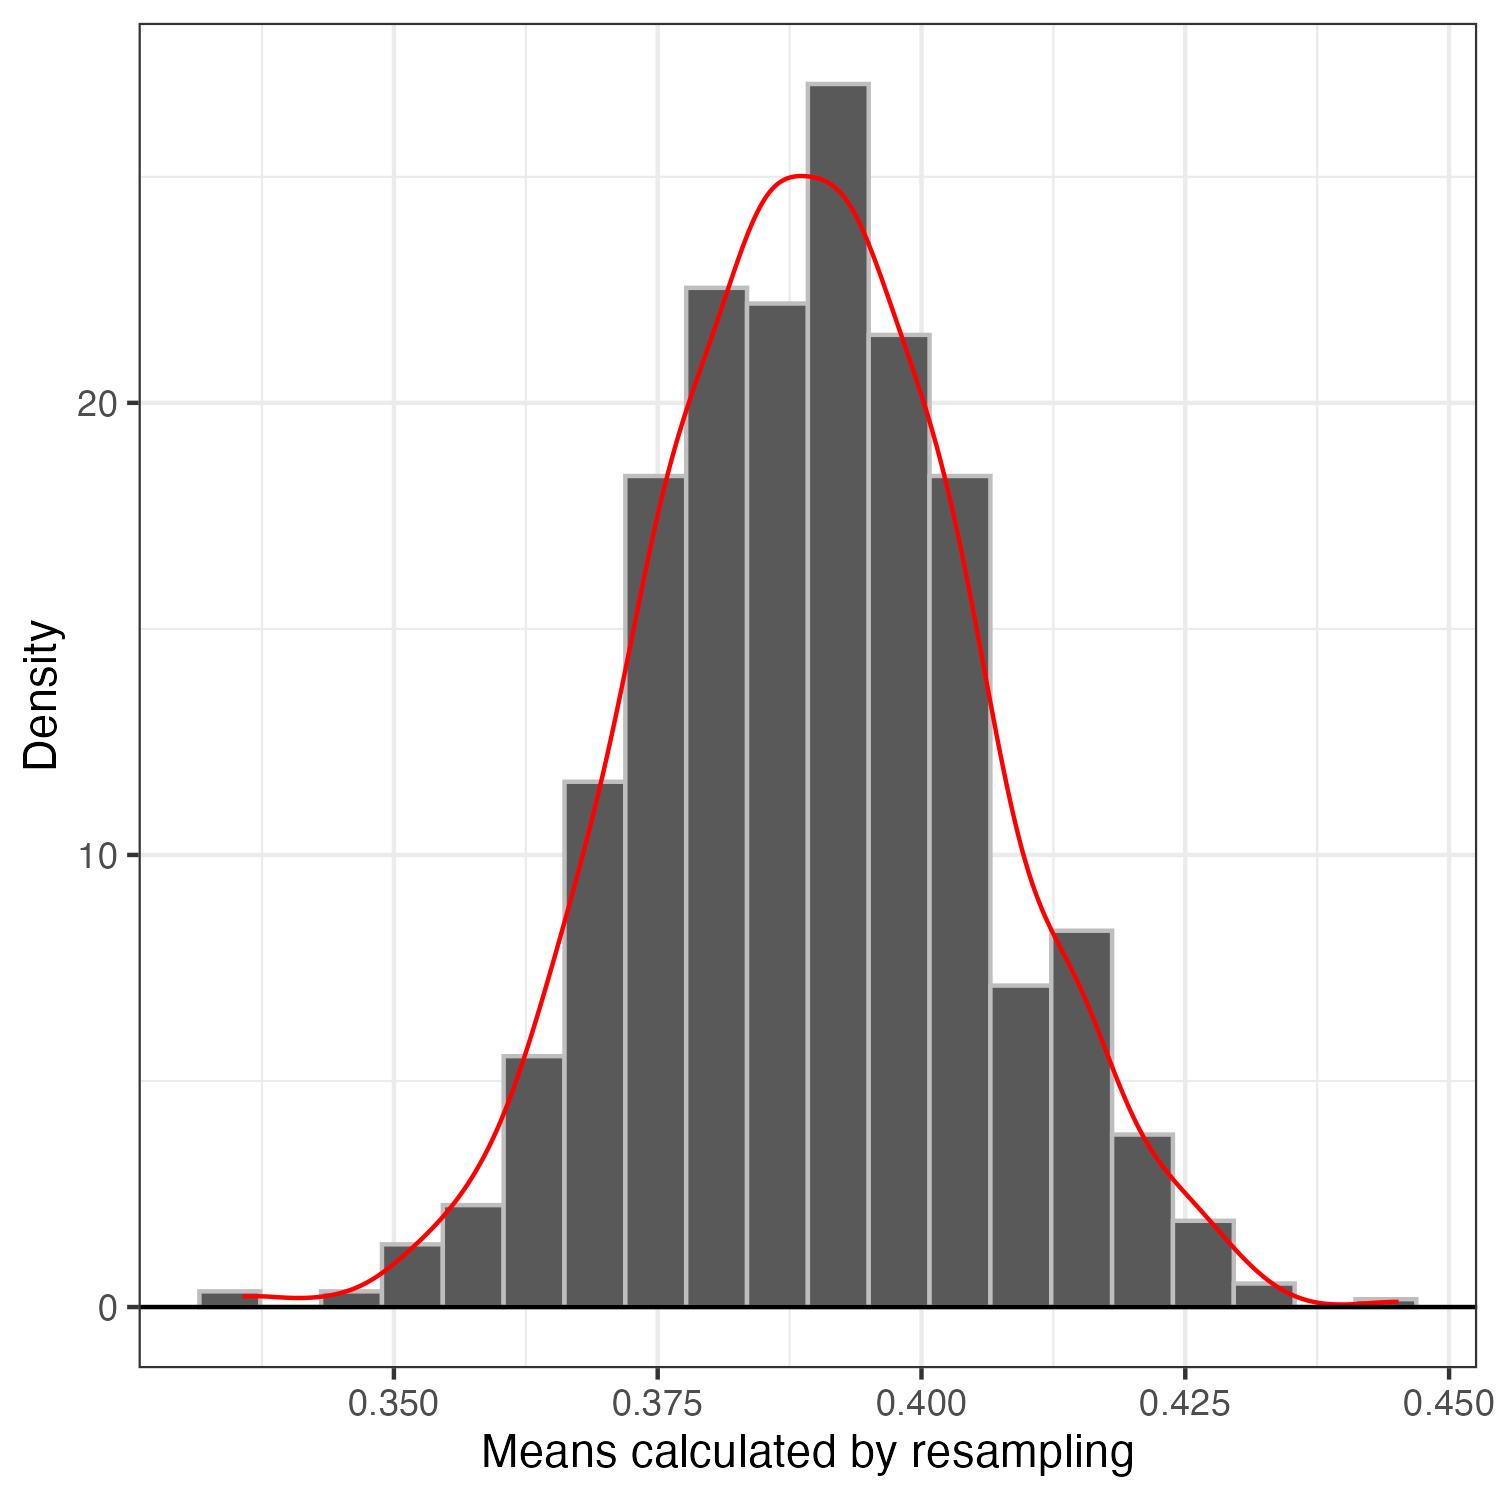
\includegraphics[width = 0.7\linewidth]{resample.png}
 \captionof{figure}{Histogram of resample proportions with superimposed density}
 \label{fig:res}
\end{Figure}

We also performed simulations for sample size $n$ in the range {100, 110, 120, ..., 3000} and the population probability proportion $p$ in the range {0.01, 0.02, ..., 0.99}. We calculated the margin of error by halving the range of the middle 95\% of observations and by using the Wilson margin of error formula.

\begin{Figure}
 \centering
 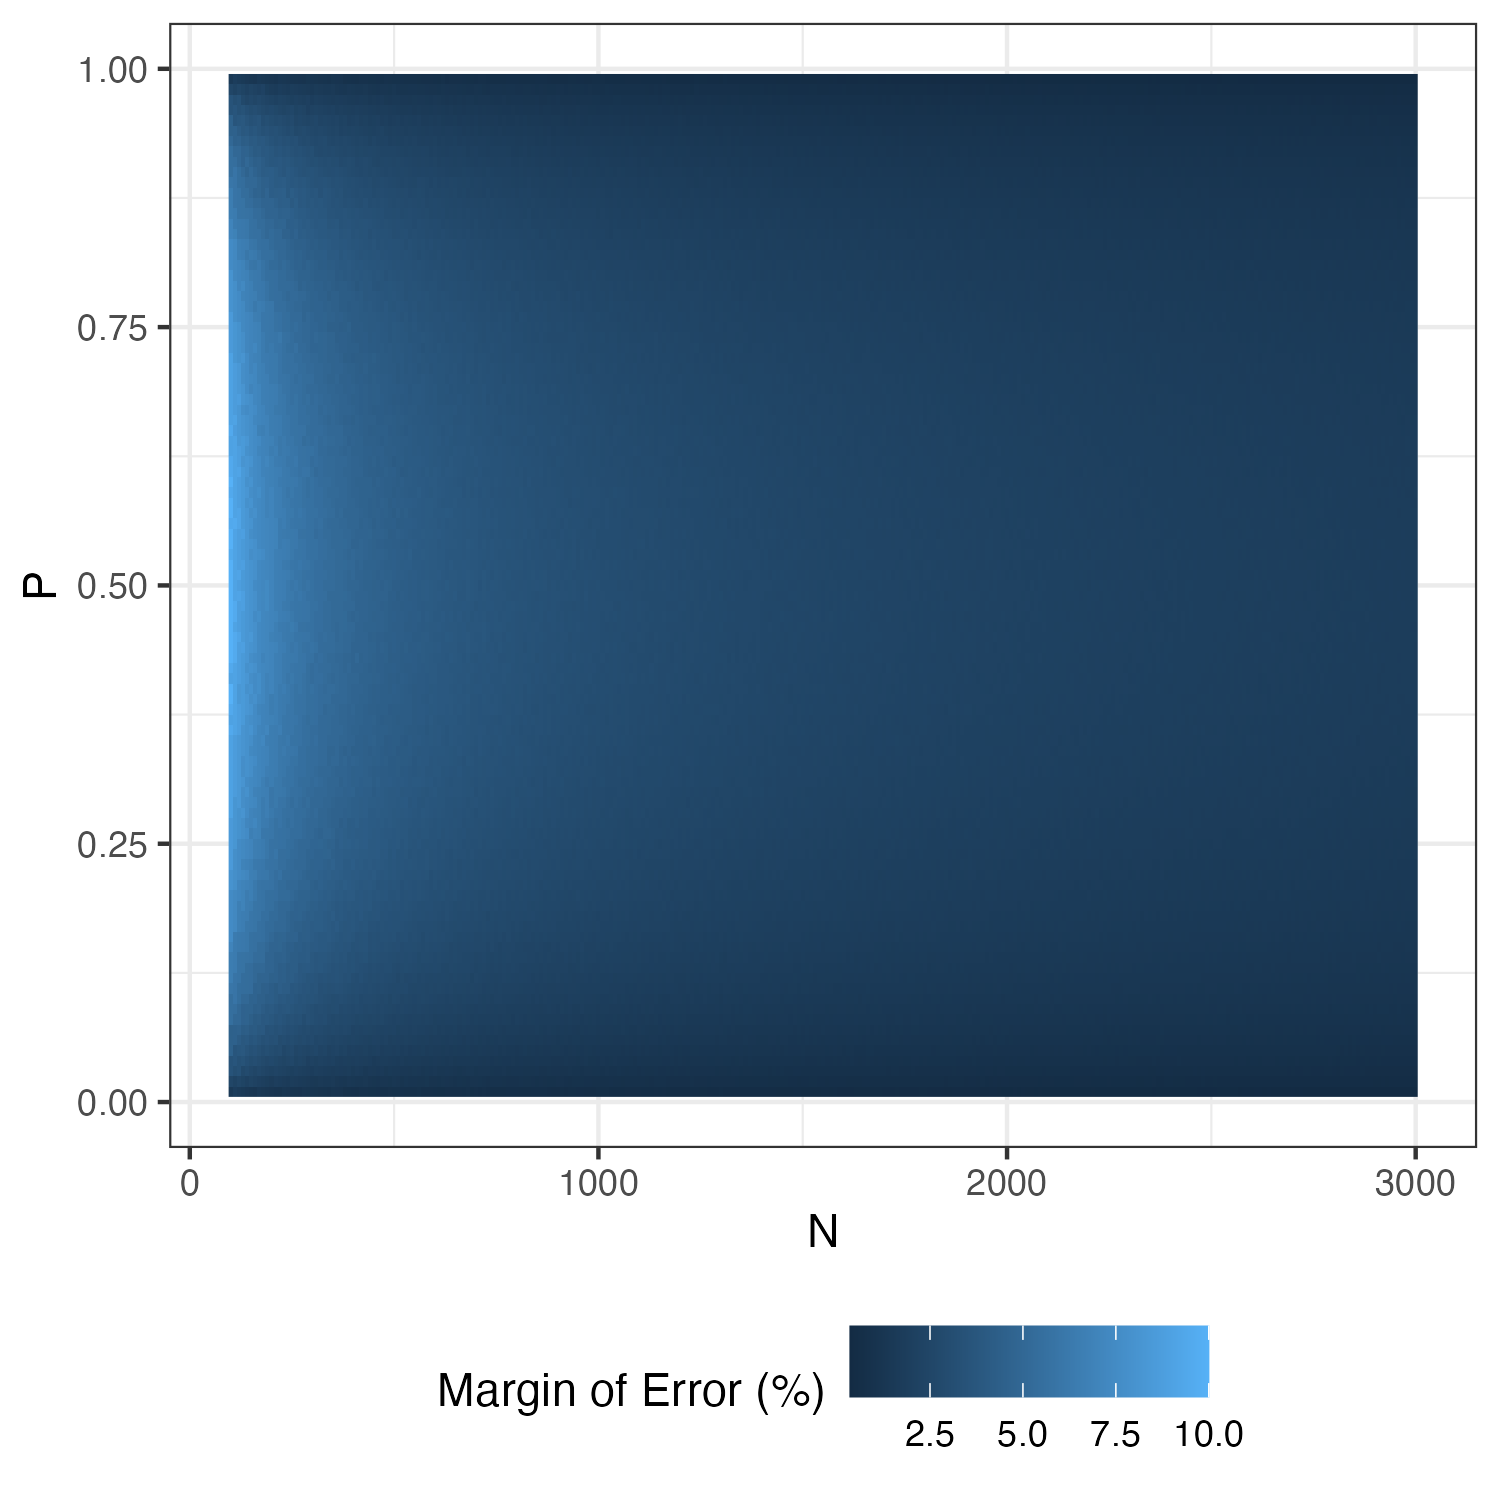
\includegraphics[width =0.7\linewidth]{error.png}
 \captionof{figure}{Estimated margin of error as a function of $n$ and $p$}
 \label{fig:err}
\end{Figure}

\begin{Figure}
 \centering
 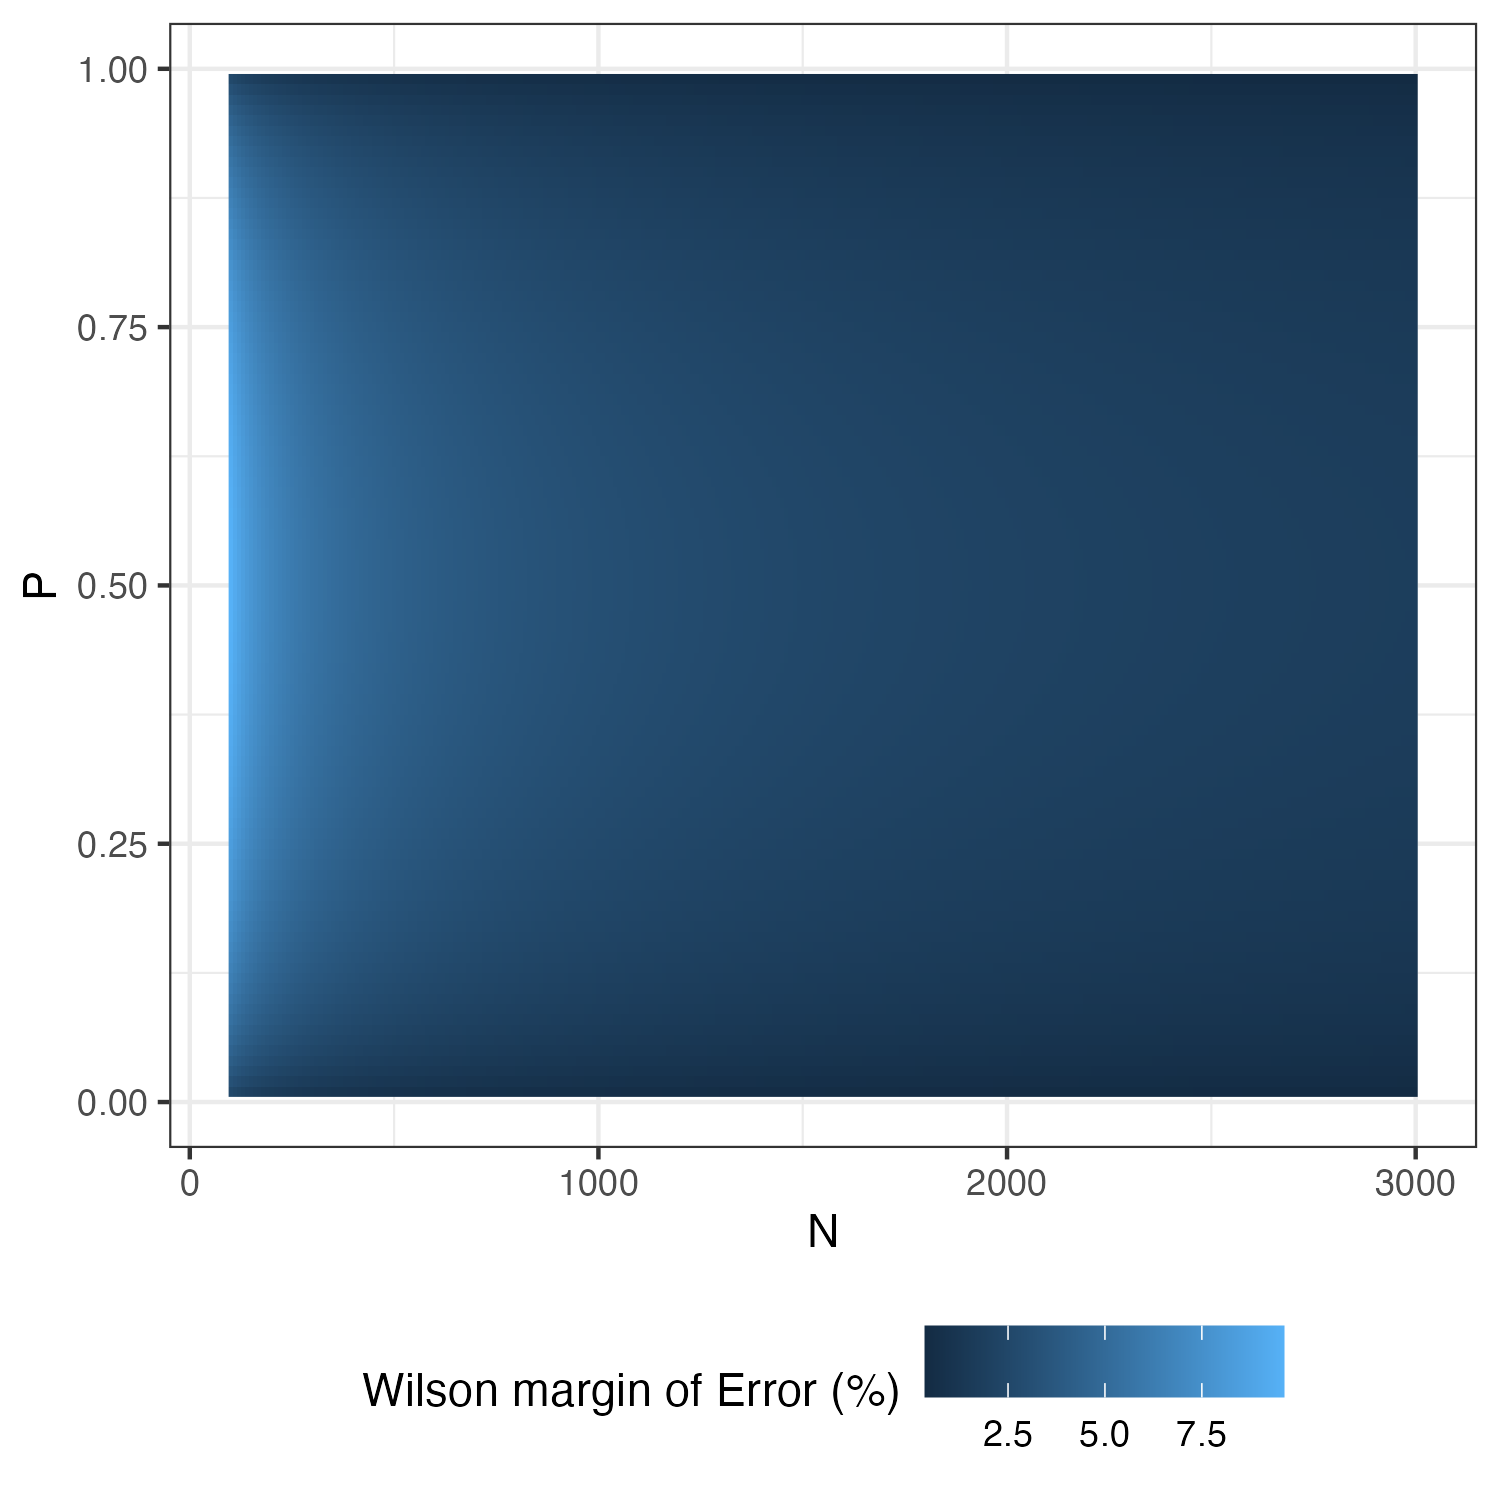
\includegraphics[width =0.7\linewidth]{error.wilson.png}
 \captionof{figure}{Estimated Wilson margin of error as a function of $n$ and $p$}
 \label{fig:errw}
\end{Figure}


\section{Results}



\section{Discussion}
 You should objectively evaluate the evidence you found in the data. Do not embellish or wish-terpet (my made-up phase for making an interpretation you, or the researcher, wants to be true without the data \emph{actually} supporting it). Connect your findings to the existing information you provided in the Introduction.

Finally, provide some concluding remarks that tie together the entire paper. Think of the last part of the results as abstract-like. Tell the reader what they just consumed -- what's the takeaway message?

%%%%%%%%%%%%%%%%%%%%%%%%%%%%%%%%%%%%%%%%%%%%%%%%%%%%%%%%%%%%%%%%%%%%%%%%%%%%%%%%
% Bibliography
%%%%%%%%%%%%%%%%%%%%%%%%%%%%%%%%%%%%%%%%%%%%%%%%%%%%%%%%%%%%%%%%%%%%%%%%%%%%%%%%
\vspace{2em}

\noindent\textbf{Bibliography:} Note that when you add citations to your bib.bib file \emph{and}
you cite them in your document, the bibliography section will automatically populate here.

\begin{tiny}
\bibliography{bib}
\end{tiny}
\end{multicols}

%%%%%%%%%%%%%%%%%%%%%%%%%%%%%%%%%%%%%%%%%%%%%%%%%%%%%%%%%%%%%%%%%%%%%%%%%%%%%%%%
% Appendix
%%%%%%%%%%%%%%%%%%%%%%%%%%%%%%%%%%%%%%%%%%%%%%%%%%%%%%%%%%%%%%%%%%%%%%%%%%%%%%%%
\newpage
\onecolumn
\section{Appendix}

If you have anything extra, you can add it here in the appendix. This can include images or tables that don't work well in the two-page setup, code snippets you might want to share, etc.

\end{document}
